% =====================================================================
% SUPPLEMENTARY MATERIAL for "Open-Vocabulary 3D Scene Graphs from Sparse Views".
% Separate PDF (ACCV allows unlimited supplementary). Holds supporting figures and the
% detailed per-class tables moved out of the 14-page main paper. Compile standalone with
% tectonic; shares figures/ assets and the palette with the main paper.
% =====================================================================
\documentclass[runningheads]{llncs}

\usepackage{booktabs}
\usepackage{graphicx}
\usepackage{amsmath}
\usepackage{amssymb}
\usepackage{tikz}
\usetikzlibrary{arrows.meta,positioning,fit,backgrounds,calc,shapes.geometric}
\usepackage{pgfplots}
\pgfplotsset{compat=1.18}
\usepgfplotslibrary{groupplots}
\usepackage{xcolor}
\usepackage[hidelinks]{hyperref}

% Shared figure palette + tikz styles.
% \input in the preamble AFTER xcolor/tikz/pgfplots are loaded.
\definecolor{cInk}{HTML}{222433}
\definecolor{cOurs}{HTML}{D9822B}     % ours / duplicate-aware dedup (amber)
\definecolor{cOursFill}{HTML}{FBE3CC}
\definecolor{cBase}{HTML}{3D5A80}     % graph-fusion baseline (steel blue)
\definecolor{cBaseFill}{HTML}{E3EAF3}
\definecolor{cUnc}{HTML}{C0392B}      % uncertainty / negative result (brick)
\definecolor{cCtrl}{HTML}{9AA0A6}     % uninformed control (grey)
\definecolor{cFrozen}{HTML}{6B82A8}   % frozen foundation models
\definecolor{cFrozenFill}{HTML}{E8EEF6}
\definecolor{cOk}{HTML}{2E7D5B}       % independent / honest (green)
\definecolor{cOkFill}{HTML}{DCEEE4}
\definecolor{cWarn}{HTML}{B5532A}     % circular / inflated (warn)
\definecolor{cWarnFill}{HTML}{F6E1D6}

% shared tikz node styles for the block diagrams
\tikzset{
  fxbox/.style={draw=cInk!70, rounded corners=2pt, align=center, font=\small,
                minimum height=8.5mm, inner sep=3.2pt, line width=0.6pt},
  frozen/.style={fxbox, draw=cFrozen, fill=cFrozenFill},
  stage/.style={fxbox, fill=gray!6},
  ours/.style={fxbox, draw=cOurs, fill=cOursFill, line width=1.1pt},
  result/.style={fxbox, draw=cOk, fill=cOkFill},
  flow/.style={-{Stealth[length=2.2mm]}, line width=0.7pt, draw=cInk!75},
}

\graphicspath{{figures/}}

% Number floats S1, S2, ... so the main paper can cite them as "Fig. S1" / "Table S1".
\renewcommand{\thefigure}{S\arabic{figure}}
\renewcommand{\thetable}{S\arabic{table}}

\begin{document}

\title{Supplementary Material\\[2pt]
\large Open-Vocabulary 3D Scene Graphs from Sparse Views via\\Duplicate-Aware Fusion and a De-Circularized Benchmark}
\titlerunning{Supplementary Material}
\author{Anonymous}
\authorrunning{Anonymous}
\institute{Anonymous}
\maketitle

This supplement holds material referenced from the main paper: the open-vocabulary detection front-end
on real frames (Fig.~\ref{fig:detections}), the duplicate-merge IoU-threshold robustness sweep
(Fig.~\ref{fig:dedup_iou}), the two detailed per-class tables (Tables~\ref{tab:perclass_overall}
and~\ref{tab:dedup_mechanism}), the full uncertainty-gate negative result
(Table~\ref{tab:uncertainty_neg}), and the per-view duplicate-aware gains with per-scene win counts
(Table~\ref{tab:dedup_delta}). All numbers match the released per-scene scores; the headline values are
already stated in the main paper.

\begin{figure}[t]
\centering
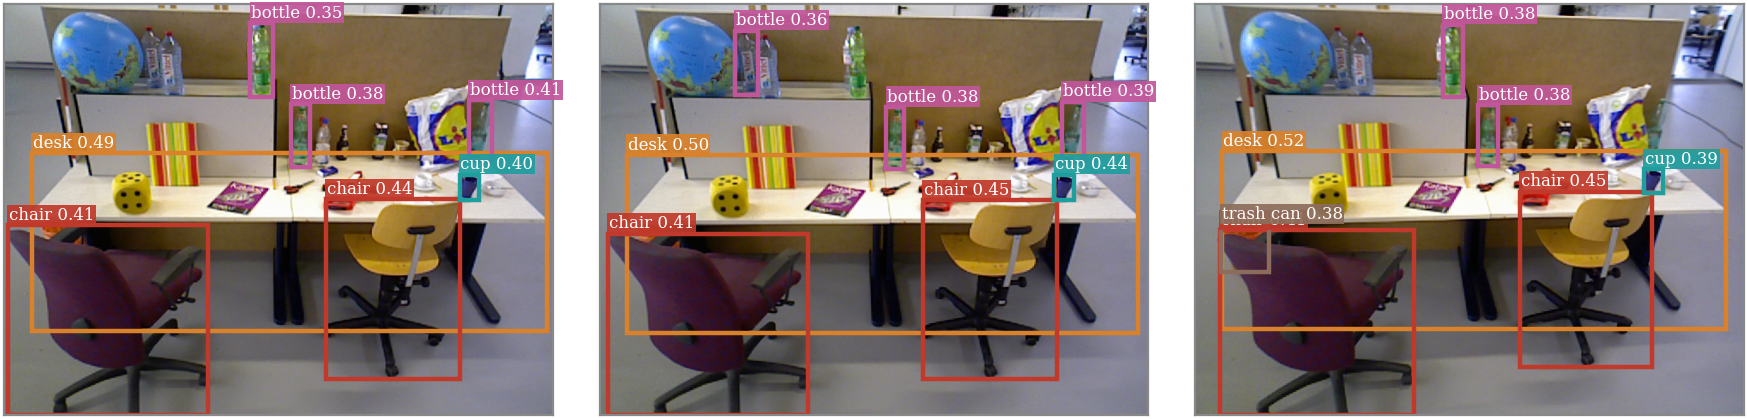
\includegraphics[width=0.88\linewidth]{fig_detections.png}
\caption{The open-vocabulary detection front-end on real frames (three views of
\texttt{freiburg3\_long\_office\_household}). OWLv2, queried with the indoor vocabulary, returns named,
boxed objects (desk, chair, bottle, cup, trash can) with confidences, the property the lifting and
fusion stages need; the common mask-then-CLIP alternative returned room-scale category noise on these
blurry frames rather than the objects present.}
\label{fig:detections}
\end{figure}


\begin{figure}[t]
\centering
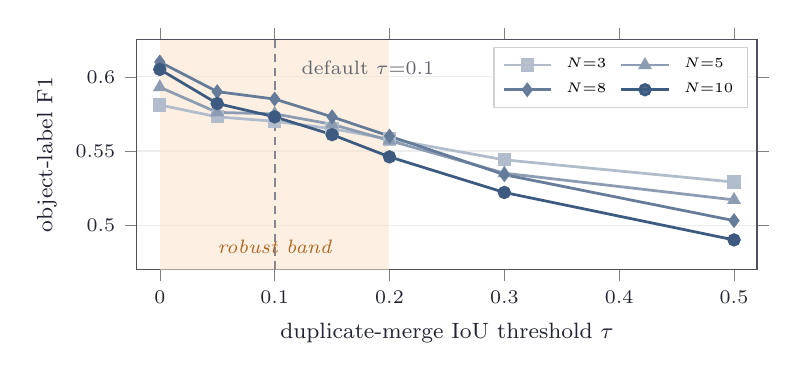
\begin{tikzpicture}
\begin{axis}[
  width=0.78\linewidth, height=4.5cm,
  xlabel={duplicate-merge IoU threshold $\tau$}, ylabel={object-label F1},
  xmin=-0.02, xmax=0.52, ymin=0.47, ymax=0.625,
  xtick={0,0.1,0.2,0.3,0.4,0.5},
  tick align=outside, axis line style={cInk!80},
  label style={font=\footnotesize, color=cInk}, tick label style={font=\scriptsize, color=cInk},
  ymajorgrids, grid style={gray!15},
  every axis plot/.append style={line width=1pt, mark size=1.9pt},
  legend style={font=\tiny, at={(0.985,0.97)}, anchor=north east, draw=gray!35,
                fill=white, fill opacity=0.9, text opacity=1, column sep=3pt, legend columns=2},
  legend cell align=left,
]
% robust low-IoU band [0, 0.2]
\fill[cOursFill, opacity=0.55] (axis cs:0,0.47) rectangle (axis cs:0.2,0.625);
% default tau = 0.1
\draw[densely dashed, cInk!55, line width=0.7pt] (axis cs:0.1,0.47) -- (axis cs:0.1,0.625);
\addplot[cBase!40, mark=square*] coordinates {(0,0.581)(0.05,0.573)(0.1,0.570)(0.15,0.565)(0.2,0.558)(0.3,0.544)(0.5,0.529)};
\addlegendentry{$N{=}3$}
\addplot[cBase!60, mark=triangle*] coordinates {(0,0.593)(0.05,0.576)(0.1,0.575)(0.15,0.568)(0.2,0.557)(0.3,0.535)(0.5,0.517)};
\addlegendentry{$N{=}5$}
\addplot[cBase!80, mark=diamond*] coordinates {(0,0.610)(0.05,0.590)(0.1,0.585)(0.15,0.573)(0.2,0.560)(0.3,0.534)(0.5,0.503)};
\addlegendentry{$N{=}8$}
\addplot[cBase, mark=*] coordinates {(0,0.605)(0.05,0.582)(0.1,0.573)(0.15,0.561)(0.2,0.546)(0.3,0.522)(0.5,0.490)};
\addlegendentry{$N{=}10$}
\node[font=\scriptsize\itshape, color=cOurs!80!black, anchor=south] at (axis cs:0.10,0.474) {robust band};
\node[font=\scriptsize, color=cInk!70, anchor=south west] at (axis cs:0.115,0.595) {default $\tau{=}0.1$};
\end{axis}
\end{tikzpicture}
\caption{Robustness of duplicate-aware fusion to the merge threshold $\tau$ (object-label F1, mean over
the 28 scenes, at $N{=}3/5/8/10$ views). The gain over \textsc{graph-fusion} is flat across the low-IoU
band $\tau\in[0,0.2]$ (average $\Delta$ from $+0.118$ at $\tau{=}0$ to $+0.075$ at $\tau{=}0.2$) and
fades only once $\tau$ is strict enough to stop merging duplicates ($+0.054$ at $\tau{=}0.3$, $+0.030$
at $\tau{=}0.5$). The default $\tau{=}0.1$ (dashed) sits within noise of the optimum.}
\label{fig:dedup_iou}
\end{figure}


\begin{table}[t]
\centering
\caption{Per-class characterization of \textsc{graph-fusion} (micro-averaged over 28 scenes, dropping
\texttt{unknown object}). Recall rises and precision falls as views are added; F1 is best at the sparse
end. The over-counting signature behind the main-paper finding.}
\label{tab:perclass_overall}
\small
\begin{tabular}{rrrr}
\toprule
Views & Precision & Recall & F1 \\
\midrule
3  & 0.519 & 0.700 & \textbf{0.596} \\
5  & 0.429 & 0.739 & 0.543 \\
8  & 0.361 & 0.794 & 0.496 \\
10 & 0.331 & 0.802 & 0.468 \\
\bottomrule
\end{tabular}
\end{table}

\begin{table}[t]
\centering
\caption{Per-class mechanism of duplicate-aware fusion at v8 (micro-averaged over 28 scenes). Dedup
recovers precision on the over-counted classes while preserving recall for almost all classes; the only
recall cost is on closely-packed same-class instances (\texttt{desk}, \texttt{bottle}).}
\label{tab:dedup_mechanism}
\small
\begin{tabular}{lccc}
\toprule
Class & \textsc{graph-fusion} P/R & dedup P/R & $\Delta$ recall \\
\midrule
\texttt{monitor}  & 0.43 / 0.95 & 0.64 / 0.95 & $0.00$ \\
\texttt{chair}    & 0.45 / 0.91 & 0.71 / 0.91 & $0.00$ \\
\texttt{floor}    & 0.27 / 0.93 & 0.71 / 0.93 & $0.00$ \\
\texttt{wall}     & 0.26 / 0.69 & 0.60 / 0.69 & $0.00$ \\
\texttt{desk}     & 0.15 / 0.96 & 0.45 / 0.92 & $-0.04$ \\
\texttt{cabinet}  & 0.36 / 0.27 & 0.67 / 0.27 & $0.00$ \\
\texttt{keyboard} & 0.39 / 1.00 & 0.50 / 1.00 & $0.00$ \\
\texttt{person}   & 0.79 / 0.79 & 1.00 / 0.79 & $0.00$ \\
\texttt{bottle}   & 0.70 / 0.76 & 0.78 / 0.72 & $-0.04$ \\
\bottomrule
\end{tabular}
\end{table}

\begin{table}[t]
\centering
\caption{Uncertainty-aware fusion is a negative result. $\Delta$ \textsc{proposed} $-$
\textsc{graph-fusion} in object-label F1 (rank-normalized, $w{=}0.3$); W/L/T is per-scene over $n=28$.
A weight sweep over $[0.1, 0.8]$ contains no setting that beats the baseline.}
\label{tab:uncertainty_neg}
\small
\resizebox{\linewidth}{!}{%
\begin{tabular}{lrrrr}
\toprule
 & v3 & v5 & v8 & v10 \\
\midrule
$\Delta$ \textsc{proposed} $-$ \textsc{graph-fusion} & $-0.033$ & $-0.053$ & $-0.082$ & $-0.096$ \\
Per-scene W/L/T                                       & 2/22/4   & 0/26/2   & 0/26/2   & 0/27/1 \\
\bottomrule
\end{tabular}
}
\end{table}

\begin{table}[t]
\centering
\caption{Duplicate-aware fusion versus the \textsc{graph-fusion} baseline and the \textsc{fixed-shrink}
control. $\Delta$ is the object-label F1 gain; W/L/T is per-scene wins/losses/ties for dedup over
\textsc{graph-fusion} ($n=28$, sign test $p<0.001$ at every view).}
\label{tab:dedup_delta}
\small
\resizebox{\linewidth}{!}{%
\begin{tabular}{lrrrr}
\toprule
 & v3 & v5 & v8 & v10 \\
\midrule
$\Delta$ dedup $-$ \textsc{graph-fusion}  & $+0.057$ & $+0.083$ & $+0.120$ & $+0.122$ \\
$\Delta$ dedup $-$ \textsc{fixed-shrink}  & $+0.065$ & $+0.101$ & $+0.141$ & $+0.154$ \\
Per-scene W/L/T (vs \textsc{graph-fusion})  & 22/1/5 & 25/0/3 & 27/0/1 & 26/1/1 \\
\bottomrule
\end{tabular}
}
\end{table}

\end{document}
